\hypertarget{convex-hull}{%
\section{Convex Hull}\label{convex-hull}}

\hypertarget{introduction}{%
\subsection{Introduction}\label{introduction}}

Given a set of points P, the Convex Hull of P, denoted conv(P) is the
smallest closed simple polygon which contains all the points in P. It
can be visualized as a tightly snapped rubber band over the given set of
points.

We would like to compute the convex hull of given set of points by using
a divide and conquer technique. Later, we will also show that the
computational complexity of our algorithm is also O(n log n). Note that
we cannot do better than is for computing convex hull

\hypertarget{how-to-run}{%
\subsection{How to Run}\label{how-to-run}}

The src folder contains the source code for the convex hull program.
\texttt{g++} from the GNU compiler suite is required to compile the
program to a executable.

Steps to Compile:

\begin{enumerate}
\def\labelenumi{\arabic{enumi})}
\tightlist
\item
  \texttt{cd} into the src directory
\item
  Run \texttt{g++\ main.cpp} which generates an executable called
  \texttt{a.out} in the same directory
\item
  Run the executable using \texttt{./a.out} (on linux)

  \begin{enumerate}
  \def\labelenumii{\arabic{enumii})}
  \tightlist
  \item
    The executable takes a dataset from command line argument. For
    example, to use an existing dataset, run
    \texttt{./a.out\ ../datasets/edge.txt}
  \item
    If no command-line argument is given, it takes input from the shell
    directly (stdin)
  \end{enumerate}
\end{enumerate}

\hypertarget{input}{%
\subsection{Input}\label{input}}

The required file format for the algorithm to work correctly is:

\begin{itemize}
\tightlist
\item
  First line must contain the no of Points to be taken as input by the
  program.
\item
  Each of next line must contain 2 integers, space seperated denoting
  the (x, y) coordinates of each point.
\item
  Each coordinate must be of integer type in the range -10\^{}6 to
  10\^{}6.
\item
  No of coordinates must be less than 1 Billion.
\item
  \textbf{Note}: while using floating point datasets, the output
  coordinates might slightly differ as given coordinates are stored as
  floats.
\end{itemize}

\hypertarget{output}{%
\subsection{Output}\label{output}}

Each line of output contains the coordinates of points present on the
convex hull in clockwise order.\\
The last two lines of output show the time taken to take input in
microseconds and the time taken by the algorithm to compute convex hull
(also in microseconds).

Example output:

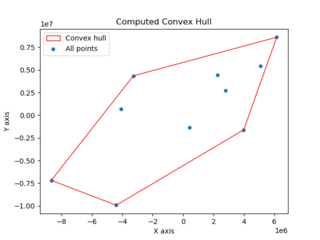
\includegraphics[width=8cm,height=8cm]{img/CH10.png}\\

\hypertarget{documentation-and-report}{%
\subsection{Documentation and Report}\label{documentation-and-report}}

Documentation of this algorithm, functions and classes can be found in
the \texttt{docs} folder in the current directory. Open the
\href{../ConvexHull/docs/html/index.html}{index.html} file from the docs
directory with your preferred browser to go through the documentation

\hypertarget{performance-analysis}{%
\subsection{Performance Analysis}\label{performance-analysis}}

Analysis is performed with a system running:

\begin{itemize}
\tightlist
\item
  OS: Arch Linux (64Bit) running Linux Kernel version 5.7.2
\item
  Processor: Intel Core i7 7700HQ
\item
  RAM: 8GB
\item
  Compiler: GNU G++ (GCC) 10.1.0
\end{itemize}

\textbf{The following observations are recorded:}

\begin{longtable}[]{@{}lcccc@{}}
\toprule
Filename & Input Dimentions & Output Diemntions & File read time &
Algorithm runtime\tabularnewline
\midrule
\endhead
edge.txt & 5 & 4 & 451 microsec & 8 microsec\tabularnewline
small.txt & 7 & 7 & 495 microsec & 16 microsec\tabularnewline
test.txt & 34 & 7 & 328 microsec & 56 microsec\tabularnewline
radial.txt & 3100 & 9 & 1348 microsec & 6.15 millisec\tabularnewline
\bottomrule
\end{longtable}

Randomly generated points (using python):

\begin{longtable}[]{@{}lcccc@{}}
\toprule
Filename & Input Dimentions & Output Diemntions & File read time &
Algorithm runtime\tabularnewline
\midrule
\endhead
10.txt & 10 & 5 & 314 microsec & 16 microsec\tabularnewline
20.txt & 20 & 7 & 495 microsec & 31 microsec\tabularnewline
50.txt & 50 & 9 & 427 microsec & 108 microsec\tabularnewline
100.txt & 100 & 13 & 348 microsec & 165 microsec\tabularnewline
500.txt & 500 & 13 & 572 microsec & 935 microsec\tabularnewline
1000.txt & 1000 (1K) & 18 & 510 microsec & 2.1 millisec\tabularnewline
3000.txt & 3000 (3K) & 24 & 2.49 millisec & 5.5 millisec\tabularnewline
5000.txt & 5000 (5K) & 22 & 2.12 millisec & 8.0 millisec\tabularnewline
10000.txt & 10000 (10K) & 23 & 3.26 millisec & 17.6
millisec\tabularnewline
50000.txt & 50000 (50K) & 28 & 17.4 millisec & 80.5
millisec\tabularnewline
100000.txt & 100000 (1L) & 31 & 39.3 millisec & 164.1
millisec\tabularnewline
250000.txt & 250000 (2.5L) & 31 & 78.1 millisec & 448.3
millisec\tabularnewline
\bottomrule
\end{longtable}

Using real world datasets:

\begin{longtable}[]{@{}lcccc@{}}
\toprule
Filename & Input Points & Output Diemntions & File read time & Algorithm
runtime\tabularnewline
\midrule
\endhead
subway-entrance-ny.txt & 1929 & 16 & 2.85 millisec & 3.81
millisec\tabularnewline
parking\_meter.txt & 15191 & 16 & 14.15 millisec & 27.04
millisec\tabularnewline
\bottomrule
\end{longtable}

Sources of datasets:

\begin{itemize}
\tightlist
\item
  \href{https://data.world/city-of-ny/5jsj-cq4s}{Parking meter dataset}
\item
  \href{https://data.world/new-york-city/subway-entrances}{New York
  Subway Entrance dataset}
\end{itemize}

It is highly difficult to calculate the time taken exactly up to the
microsecond, hence the value might vary on different executions. Also,
please note that the time calculated here may vary based on the system
load and other background applications.

\hypertarget{algorithm-approach}{%
\subsection{Algorithm Approach}\label{algorithm-approach}}

For more detailed information regarding the algorithm, refer to David
Mount Lecture notes from the course
\href{https://www.cs.umd.edu/class/spring2020/cmsc754/lectures.html}{CMSC
754 - Computational Geometry}

Given set of points P, we would like to first order them according to
the increasing x coordinate. For the sake of simplicity, let us assume
that no two points will have same x or y coordinate and no 3 points are
co-linear.

First, we will recursively compute the upper hull and then similarly
compute the lower hull of the given set of points. Finally, we will join
the upper hull with the lower hull to complete the convex hull and
return/print the clockwise ordering of the points present on the convex
hull

\textbf{Upper Hull Computation}

We divide the input set of points into 2 equal halves and recursively
compute the upper hull for both the half. Then, we compute the upper
tangent to both the hulls by traversing from the right on left hull and
traversing from left on the right hull. We perform orientation tests to
determine when the orientation changes on each hull respectively and
move upwards a point. We perform this operations until we reach the
upper part of both hulls.

All the traversed points on both hulls except the one which lead to
tangent are deleted (because all of them lie under tangent, hence lie
inside the polygon) and the resulting points of both hulls are catenated
to get the upper hull.

\hypertarget{results}{%
\subsection{Results}\label{results}}

The following is the computed convex hull of the
\href{./datasets/parking_meter.txt}{parking\_meter.txt} dataset:

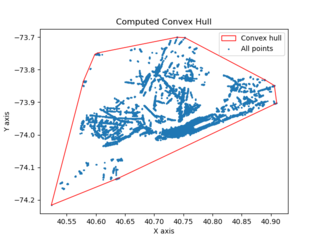
\includegraphics[width=8cm,height=8cm]{img/CHparkingmeter.png}\\

The red boundary in the above image represents the convex hull given as
the output by the program. The blue points are the inputs given to the
program.

By analysis of the above divide and conquer algorithm, It can be
concluded that the algorithm runs in O(n log n) time complexity. From
the above results of testing of various datasets, we can see that the
time increase is proportional to the no of points.

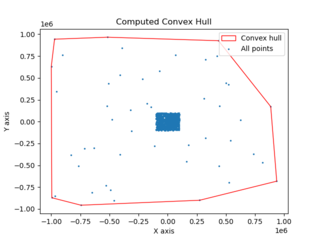
\includegraphics[width=8cm,height=8cm]{img/CHradial.png}\\

The dataset \href{./datasets/radial.txt}{radial.txt} is a hand-crafted
dataset (3K points) which has high concentration of points
(\textasciitilde2.1K) in the center, whereas other randomly generated
datasets (for example: \href{./datasets/3000.txt}{3000.txt})have a
uniform distribution of points (the python random number generator uses
an underlying uniform distribution). From this we can assume that
independant of positioning of points, our algorithm takes approximately
the same time to compute the convex hull.

\hypertarget{conclusion}{%
\subsection{Conclusion}\label{conclusion}}

For the last dataset which contains 2.5L points, its worth noting that
the algorithm runs in just under 500ms which might appear to be fast.
But for applications like graphics, rendering and animations, this poses
a huge overhead in terms of repeated computation of convex hull for
various objects.

One observation we can make here is that the number of points which are
present on the convex hull is usually relatively lower most of the
times. So, using an output sensitive algorithms (Ex: Jarvis's march)
might help us if our application has fewer vertices on the convex hull.

It's worth noting that convex hull computation cannot be done under O(n
log n) which has been proved. Therefore, we can only hope to reduce the
constants of complexity. In our algorithm, we repeatedly recurse, hence
make many function calls which is computationally expensive. Hence by
using algorithms like Chan's or Grahm's, we can do better
